\documentclass[11pt, a4paper]{article}
\usepackage{graphicx, fullpage, hyperref, listings}
\usepackage{appendix, pdfpages, color}
\usepackage{indentfirst} %段首空两格 棒
\usepackage{chngpage} 
\usepackage{tocloft}            % This squashes the Table of Contents a bit
\usepackage{pdfpages}
\usepackage{multirow}
\usepackage{amsmath}
\usepackage{framed}

\setlength\cftbeforesecskip{3pt}
\renewcommand{\contentsname}{\centerline{\textbf{Content}}}
\graphicspath{{images/}}

\usepackage{multicol}

\usepackage{graphicx}
\usepackage{epstopdf}
\hypersetup{CJKbookmarks,%
	bookmarksnumbered,%
	colorlinks,%
	linkcolor=black,%
	citecolor=black,%
	plainpages=false,%
	pdfstartview=FitH}

%%%%%%%代码语法高亮设置

\usepackage{color}

\definecolor{pblue}{rgb}{0.13,0.13,1}
\definecolor{pgreen}{rgb}{0,0.5,0}
\definecolor{pred}{rgb}{0.9,0,0}
\definecolor{pgrey}{rgb}{0.46,0.45,0.48}

\usepackage{listings}
\lstset{
	language=Java,
	showspaces=false,
	showtabs=false,
	%%%%%
	frame = single,
	stepnumber = 2,  
	numbersep = 4pt, 
	 numbers=left,
	%breakatwhitespace=false, 
	tabsize=2,  
	%%%%%
	breaklines=true,
	showstringspaces=false,
    breakatwhitespace=false, 
	commentstyle=\color{pgreen},
	keywordstyle=\color{pblue},
	stringstyle=\color{pred},
	basicstyle=\ttfamily,
	%moredelim=[il][\textcolor{pgrey}]{$$},
	%moredelim=[is][\textcolor{pgrey}]{\%\%}{\%\%},
}


%%%%%%%%代码语法高亮设置

\definecolor{MyLightYellow}{cmyk}{0,0.,0.2,0} 

\setlength{\parskip}{4pt}        % sets spacing between paragraphs
\interfootnotelinepenalty=500    % this prevents footnotes breaking across pages

\title{
\includegraphics[width=0.45\textwidth]{wpi2}
        \\CS 539: Machine Learning \\ 
    Project Proposal }          % <<<<<<<<< change the title as appropriate
\author{}                                    % <<<<<<<<< module code
\date{\today}



\begin{document}


\begin{titlepage}
\maketitle
\addtocontents{toc}{\protect\thispagestyle{empty}} % because we don't want a page number on the title page
% Thanks to Huang Shanyue for suggesting this 

\begin{center}
	Group Member
\end{center}

\begin{table}[htbp] 
	\begin{center}
		\begin{tabular}{l l l} 
			
			Yu & Li  &   yli14@wpi.edu \\
			Ruojun & Li  &   rli2@wpi.edu \\
			Jiaming & Nie  &  jnie@wpi.edu \\
			Yang & Tao   &  ytao2@wpi.edu \\
			Guangda & Li &    gli5@wpi.edu    \\
		\end{tabular}
	\end{center}
\end{table}


 
%\fbox{
%I confirm that I have read and understood the University’s Academic Integrity Policy. \\
 
%I confirm that I have acted honestly, ethically and professionally in conduct leading to assessment for the programme of study. \\

%I confirm that I have not copied material from another source nor committed plagiarism nor fabricated, falsified or embellished data when completing the attached piece of work. I confirm that I have not copied material from another source, nor colluded with any other student in the preparation and production of this work.  \\

%SIGNATURE Jiaming Nie \\

%DATE \date{\today}

% Unless this is written out, word for word, your report cannot be accepted.
%\end{minipage}
%}

\thispagestyle{empty}  %去除首页页码

\end{titlepage}

%\tableofcontents
%\listoffigures

%\newpage

\section{Abstract}

Style transfer is the technique for recomposing images in the style of other images. With the development of deep learning in the computer vision field, style transfer has been popular with the applications of CNN (Convolutional Neural Network). In this project, our group will build a real-time image style transfer project using CNN.

\section{Problem Statement}

The goal of this project is to implement a real-time image style transfer demonstration using deep learning. One deep CNN will be used to learn the style of the input image and then output the content image which learns the style of the style image. Style transfer can be defined as finding a pastiche image $p$ whose content is similar to that of a content image $c$ but whose style is similar to that of a style image $s$~\cite{ref:source1}. 

The neural algorithm of neural style transfer proposes the definitions following~\cite{ref:source1}:

\begin{itemize}
\item Two images are similar in content if their high-level features are extracted by a trained classifier are close in Euclidian distance;
\item Two images are similar in style if their low-level features as extracted by a trained classifier
share the same statistics or, more concretely, if the difference between the features' Gram
matrices has a small Frobenius norm.
\end{itemize}

In the training of the CNN there will be the content and style reconstruction with the combinations of the output of different convolutional layers~\cite{ref:source2}.

The flowchart of the neural style transfer is illustrated in figure~\ref{fig:nst-demo}:

\begin{figure}[htbp]
	\centering %使插入的图片居中显示
	
	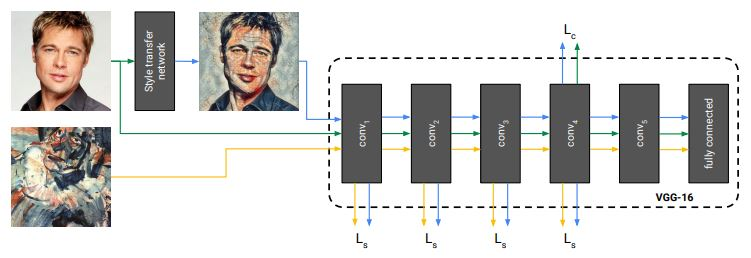
\includegraphics[width=8cm]{image1}
	\caption{Neural Style Transfer Demonstration~\cite{ref:source1}\cite{ref:source2}}
	\label{fig:nst-demo}
	%插入图片的标题,一般放在图片的下方,放在表格的上方
\end{figure}

\section{Motivation}

Neural style transfer has been popular for recent years with the application of Deep CNN. The Multi-style transfer with the training with deep neural network has also been applied in the area of computer vision. The motivation of this project is to implement the real-time neural style transfer with the integration of openCV. 

OpenCV has provided the state-of-art image processing and computer vision tools for the prerequisite processing functions to process the input style image for the CNN and then output content image. The project will train the COCO image datasets and to implement multi-style style transfer. 

\section{Hypothesis}

The implementations of multi-style transfer in the training Deep CNN is to obtain the convergence of the loss function. In the neural style transfer, the loss function is given on the following with the initialization of $p$ and $c$ from certain type Gaussian Noise as stated in the problem statement part and the algorithm adapts $p$ to minimize the loss function $\mathcal{L}$~\cite{ref:source3} in equation~\ref{eq:eq1}:

\begin{equation}
\label{eq:eq1}
\mathcal{L}(s,c,p) = \lambda_{s}\mathcal{L}_{s}{p} + \lambda_{c}\mathcal{L}_{c}{p}
\end{equation} 

$\mathcal{L}_{s}{p}$ is the style loss and $\mathcal{L}_{c}{p}$ is the content loss and $\lambda_{s}$, $\lambda_{c}$ are scaling hyperparameters. The style and content losses are defined as in equation~\ref{eq:eq2}\ref{eq:eq3} with style layers $\mathcal{S}$ and content layers $\mathcal{C}$ are given. 
 
\begin{equation}
\label{eq:eq2}
\mathcal{L}_{s}(p) = \sum_{i\in \mathcal{S}} \frac{1}{U_{i}} || G(\phi_{i}(p)) - G(\phi_{i}(s)) {||}^{2}_{F}
\end{equation} 

\begin{equation}
\label{eq:eq3}
\mathcal{L}_{s}(p) = \sum_{j\in \mathcal{C}} \frac{1}{U_{j}} ||\phi_{j}(p) - \phi_{j}(c) {||}^{2}_{F}
\end{equation} 

The style transfer network $T$ is a feed-forward convolutional network which takes content image $c$ and outputs the pastiche image $p$ directly. The loss function then can be reduced to equation~\ref{eq:eq4}.

\begin{equation}
\label{eq:eq4}
\mathcal{L}{s,c} = \lambda_{s}\mathcal{L}(T(c)) + \lambda_{c}\mathcal{L}(T(c)) 
\end{equation} 
 
\section{Deliverable}

This project will rely on the training of the deep style transfer neural network and the graphical user interface to integrate the OpenCV and the pre-trained neural network to perform the function. 

A graphical user interface will integrate different function blocks.


\section{Summary}

The project will implement the neural style transfer with the training of deep CNN. The timetable of the project is on the following:

\begin{itemize}
\item Oct. 27th: Submit Project Proposal 
\item Dec. 5th: Demo Website 
\item Dec. 6th/13th: Project Presentation
\end{itemize}


%\tableofcontents

%\listoffigures
%\listoftables
%\lstlistoflistings        


\newpage
\bibliographystyle{IEEEtran}  
\bibliography{MyRefs} 
\addcontentsline{toc}{section}{References}





%-------------------------------------------------------------------------------------------------------





\end{document}
